\documentclass{sig-alternate}
\usepackage{url}
\usepackage{graphicx}
\usepackage{subfigure}
\usepackage{hyperref}
\usepackage{url}
\usepackage{times}
\usepackage{balance}
\usepackage{xspace}
\usepackage{paralist}
\usepackage{relsize}

%\usepackage{xfrac}

\conferenceinfo{MSR}{'14, May 31 -- June 1, 2014, Hyderabad, India}
\CopyrightYear{2014}
\crdata{978-1-4503-2863-0/14/05}

\begin{document}

\newcommand{\todo}[1]{\textbf{TODO}\footnote{\textbf{TODO:} #1}}

\newcommand{\ghtorrent}{\textsc{ght}orrent\xspace}
\newcommand{\api}{\textsc{api}\xspace}
\newcommand{\pullreqs}{\textsf{pullreqs}\xspace}

\title{A Dataset for Pull-Based Development Research}
\numberofauthors{2}

\author{
\alignauthor
Georgios Gousios\\
       \affaddr{Delft University of Technology}\\
       \affaddr{Delft, the Netherlands}\\
       \email{g.gousios@tudelft.nl}
\and
Andy Zaidman\\
       \affaddr{Delft University of Technology}\\
       \affaddr{Delft, the Netherlands}\\
       \email{a.e.zaidman@tudelft.nl}
}

\maketitle

\begin{abstract}

Pull requests form a new method for collaborating in distributed software
development. To study the pull request distributed development model, we
constructed a dataset of almost 900 projects and 350,000 pull requests,
including some of the largest users of pull requests on Github. In this paper,
we describe how the project selection was done, we analyze the selected features
and present a machine learning tool set for the R statistics environment. 

\end{abstract}

\category{D.2.7}{Software Engineering}{Distribution, Maintenance, and Enhancement}[Version control]
\category{D.2.9}{Software Engineering}{Management}[Programming teams]

\terms{Management}

\keywords{pull-based development, pull request, distributed software development,
empirical software engineering}

\section{Introduction}
\label{sec:intro}

Pull requests as a distributed development model in general, and as implemented
by Github in particular, form a new method for collaborating on distributed
software development. In the pull-based development model, the project's main
repository is not shared among potential contributors; instead, contributors
\emph{fork} (clone) the repository and make their changes independent of each
other. When a set of changes is ready to be submitted to the main repository,
they create a pull request, which specifies a local branch to be merged with a
branch in the main repository. A member of the project's core team is then
responsible to inspect the changes and pull them to the project's master branch.
If changes are considered unsatisfactory, more changes may be requested; in that
case, contributors need to update their local branches with new commits.
Furthermore, as pull requests only specify branches from which certain commits
can be pulled, there is nothing that forbids their use in the shared 
repository approach (cross-branch pull requests).

To understand what the underlying principles that guide pull-based development
are, we created \pullreqs, a curated dataset of almost 900 projects along with a
set of tools for its analysis. A previous version of the dataset has been used
to quantitatively study the pull request development process~\cite{GPD14}. The
\pullreqs dataset is based on our previous work on \ghtorrent~\cite{Gousi13},
albeit only for its construction. While \ghtorrent is a full mirror of all
data offered by the Github {\sc api}, the \pullreqs dataset includes many features extracted by combining \ghtorrent and the project's repository; the dataset is offered in a format ready to be processed by statistical software.
In this paper, we describe the construction
process of the dataset and outline directions for further research with it.

\section{Feature Selection}
\label{sec:expdata}

The feature selection was based on prior work in the areas of patch submission
and acceptance~\cite{Nagap05,Bird07a,Weiss08,Baysa12}, code
reviewing~\cite{Rigby13}, bug triaging~\cite{Anvik06, Giger10} and also
on semi-structured interviews of Github developers~\cite{Dabbi12, Pham13}. The
selected features are split into three categories:

  \emph{Pull request characteristics.} These features attempt to quantify the
  impact of the pull request on the affected code base. When examining external
  code contributions, the size of the patch is affecting both acceptance and
  acceptance time~\cite{Weiss08}. There are various metrics to determine the
  size of a patch that have been used by researchers: code churn~\cite{Nagap05},
  changed files~\cite{Nagap05} and number of commits.  In the particular case of
  pull requests, developers reported that the presence of tests in a pull
  request increases their confidence to merge it~\cite{Pham13}. To investigate
  this, we split the churn feature into two features, namely \texttt{src\_churn}
  and \texttt{test\_churn}. The number of participants has been shown to
  influence the time required to do a code review~\cite{Rigby13}. Finally,
  through our own experience analyzing pull requests, we have found that in many
  cases conflicts are reported explicitly in pull request comments while in
  other cases pull requests include links to other related pull requests. We
  therefore included corresponding binary features in the dataset.

  \emph{Project characteristics.} These features quantify how receptive to pull
  requests a project is. If the project's process is open to external
  contributions, then we expect to see an increased ratio of external
  contributors over team members. The project's size may be a detrimental factor
  to the speed of processing a pull request, as its impact may be more difficult
  to assess. Also, incoming changes tend to cluster over time (the ``yesterday's
  weather'' change pattern), so it is natural to assume that pull
  requests affecting a part of the system that is under active development will
  be more likely to merge. Testing plays a role in speed of processing;
  according to~\cite{Pham13}, projects struggling with a constant flux of
  contributors use testing, manual or preferably automated, as a safety net to
  handle contributions from unknown developers.

  \emph{Developer.}  Developer-based features quantify the influence that the
  person who created the pull request has on the decision to merge it and the
  time to process it. In particular, the developer who created the patch has
  been shown to influence the patch acceptance decision~\cite{Jeong09}. To
  abstract the results across projects with different developers, we include
  features that quantify the developer's track record~\cite{Dabbi12}, namely the
  number of previous pull requests and their acceptance rate; the former has
  been identified as a strong indicator of pull request quality~\cite{Pham13}.
  Bird et al.~\cite{Bird07}, presented evidence that social reputation has an
  impact on whether a patch will be merged; in our dataset, the number of
  followers on Github can be seen as a proxy for reputation.

All features must be calculated at the time a pull request has been closed or
merged, to evaluate the effect of intermediate updates to the pull request as a
result of the ensuing discussion. Features that contain a temporal dimension in
their calculation (e.g., \texttt{team\_size} or
\texttt{commits\_on\_files\_touched}) are calculated over the three-month time
period before the pull request was opened.

The full list of features can be seen in Table~\ref{tab:features}.


\section{Dataset Construction}

The distribution of pull requests per project in Github is extremely skewed
(quantiles 5\%: 1, 95\%: 68, mean: 26, median: 4). By the end of 2013, 255,914
projects had received a pull request while only 8,600 had received more than
100. To ensure that the selected projects used pull requests as part of the
project development cycle, rather than just occasional external contributions,
we only selected the top 1\% of projects by total number of pull requests
created. The initial selection led to 2,551 projects.
In addition, to evaluate testing related features as described above,
we needed a way to determine whether a source code file in a project
repository represented test code.
For that, we exploited the
convention-based project layout in the Ruby (Gem), Python, Java and Scala (both
Maven) language ecosystems, so our project selection was limited to those
languages. 1,517 projects where thus filtered out.

For the remaining 1,034 repositories, the full history (including pull requests,
issues and commits) of the included projects was downloaded and features were
extracted by querying the \ghtorrent databases and analyzing each project's Git
repository.

\begin{figure}
  \begin{center}
    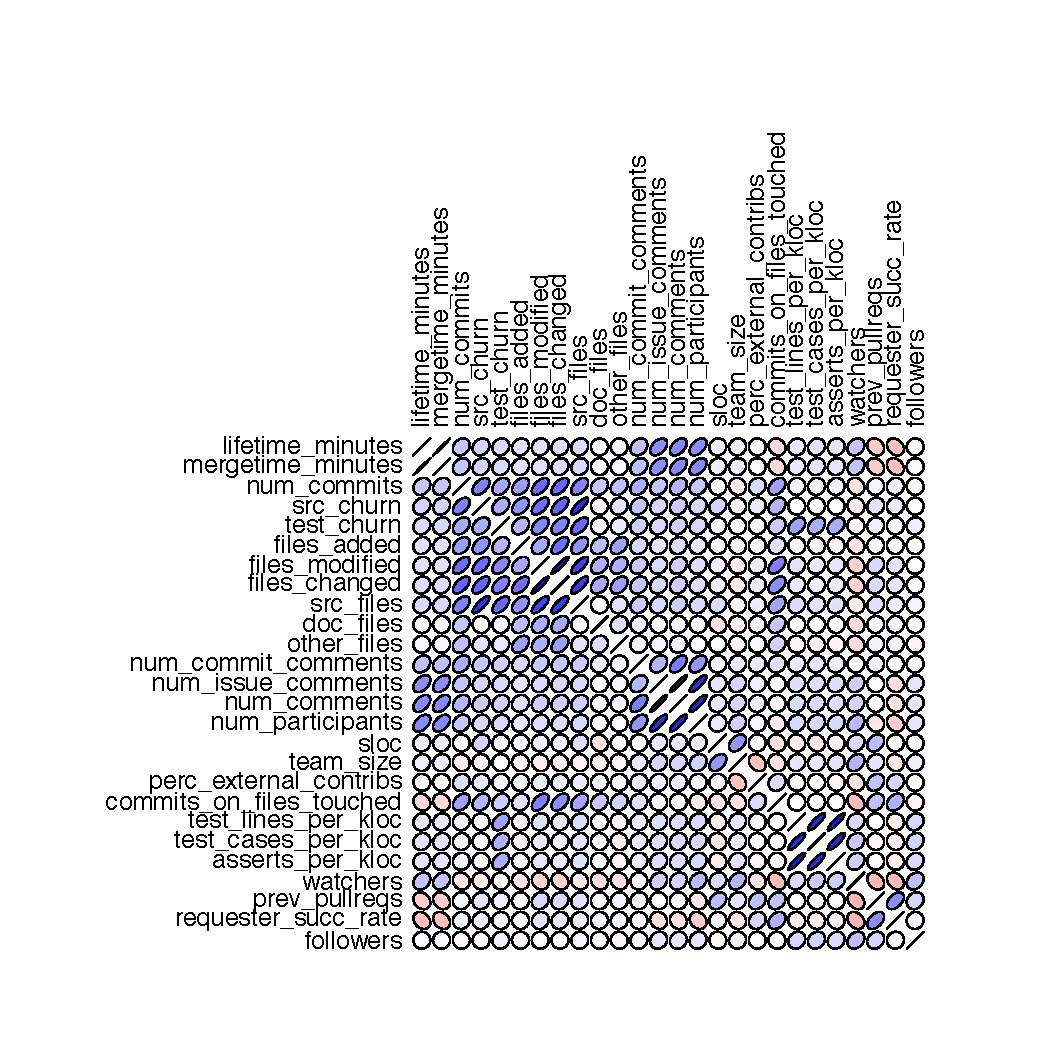
\includegraphics[scale=0.6]{cross-cor.pdf}
  \end{center}
  \caption{Cross-correlation (Spearman) among all dataset features. Blue color (or right slant) indicates positive correlation, red color (or left slant) is negative correlation. The darker the color, the stronger the correlation.}
  \label{fig:features}
\end{figure}

\begin{table*}[ht]
\centering
\caption{Selected features and descriptive statistics. Histograms are in log scale.} 
\begin{small}
\begin{tabular}{rp{24em}rrrrl}
  \hline
  \bfseries{Feature} & \bfseries{Description} & \bfseries{5 \%} & \bfseries{mean} & \bfseries{median} & \bfseries{95 \%} & \bfseries{Histogram} \\ 
  \hline

  \multicolumn{2}{l}{\bf{Pull Request Characteristics}}\\

  \texttt{num\_commits} & Number of commits in the pull request & 1.00 & 4.47 & 1.00 & 12.00 & 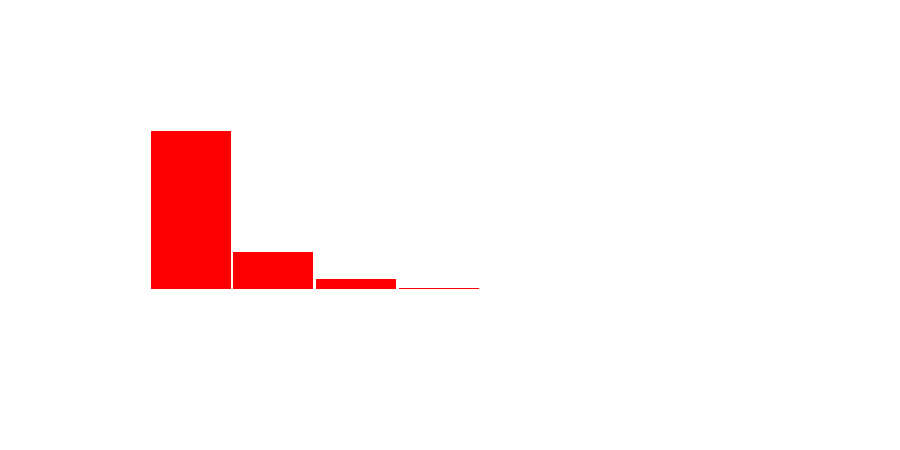
\includegraphics[scale = 0.1, clip = true, trim= 50px 60px 50px 60px]{hist-f128f3cb38588fe5202716588c047381.pdf} \\ 
  \texttt{src\_churn} & Number of lines changed (added + deleted) by the pull request. & 0.00 & 300.72 & 10.00 & 891.00 & 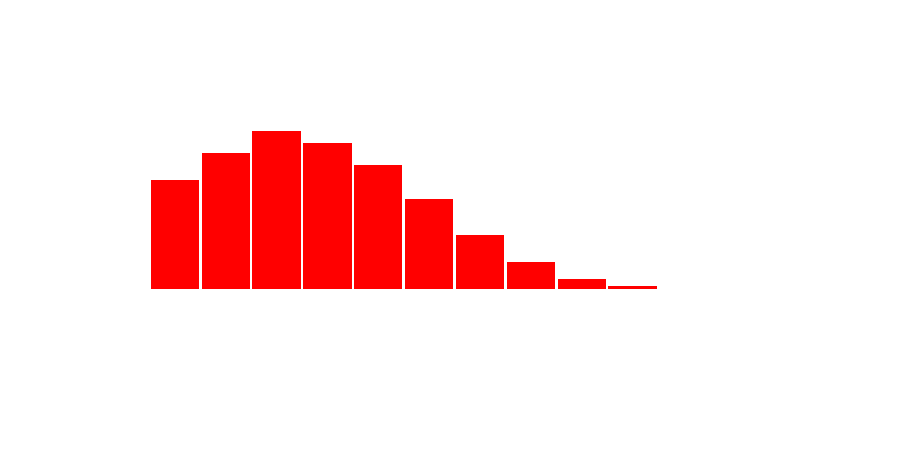
\includegraphics[scale = 0.1, clip = true, trim= 50px 60px 50px 60px]{hist-1f006c80a0da61518435a0c55f538326.pdf} \\ 
  \texttt{test\_churn} & Number of test lines changed in the pull request. & 0.00 & 88.88 & 0.00 & 282.00 & 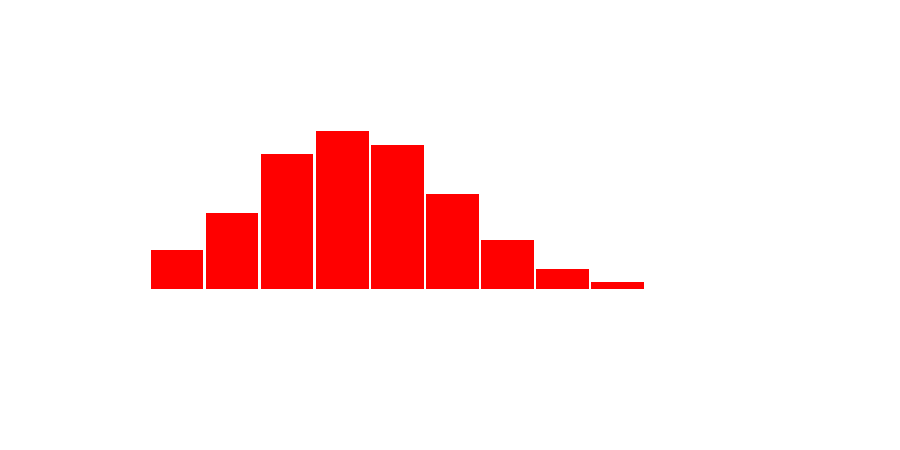
\includegraphics[scale = 0.1, clip = true, trim= 50px 60px 50px 60px]{hist-dd78ccaeedd7fc79735a66eb7f9e506b.pdf} \\ 
  \texttt{files\_changed} & Number of files touched by the pull request. & 1.00 & 12.12 & 2.00 & 31.00 & 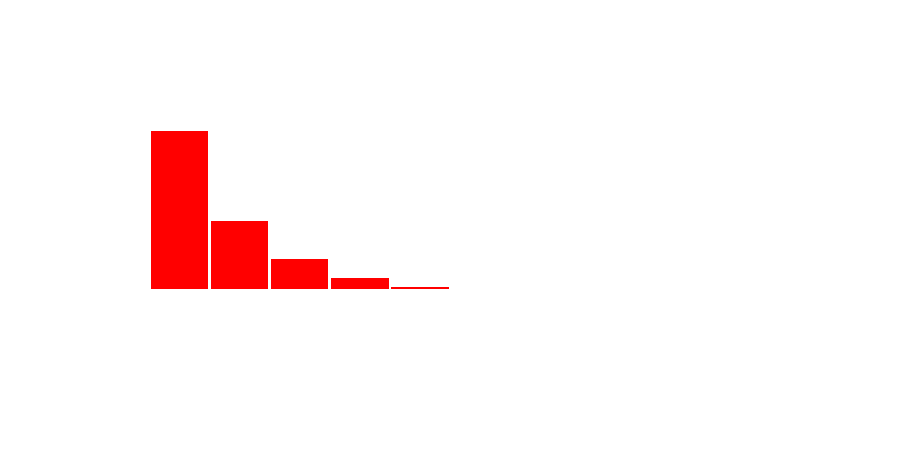
\includegraphics[scale = 0.1, clip = true, trim= 50px 60px 50px 60px]{hist-9b07b060359435635ff2bf4cd34f834a.pdf} \\ 
  \texttt{num\_comments} & Discussion and code review comments. & 0.00 & 2.77 & 1.00 & 12.00 & 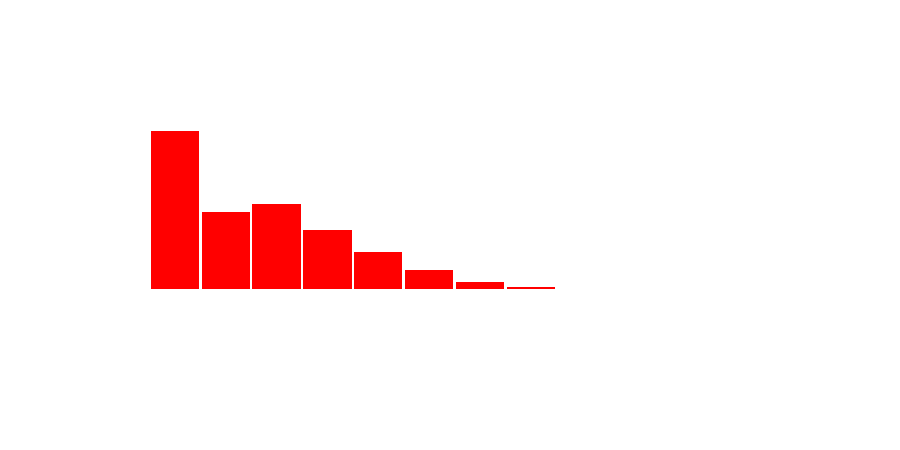
\includegraphics[scale = 0.1, clip = true, trim= 50px 60px 50px 60px]{hist-9db5e2b390de0d64d26c14798cb579ef.pdf} \\ 
 
  \texttt{num\_participants} & Number of participants in the pull request discussion & 0.00 & 1.33 & 1.00 & 4.00 & 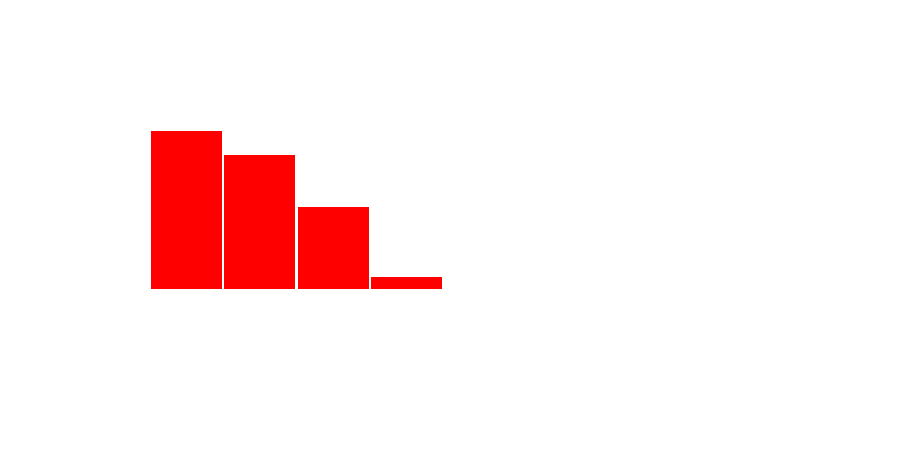
\includegraphics[scale = 0.1, clip = true, trim= 50px 60px 50px 60px]{hist-7d419bb69f175ea7015a9bdc71172f38.pdf} \\

  \texttt{conflict} & The word \emph{conflict} appears in the pull request comments.  & --- & --- & --- & --- & ---\\

    \texttt{forward\_link} & Pull request includes links to other
    pull requests. & --- & --- & --- & --- & --- \\


  \multicolumn{2}{l}{\bf{Project Characteristics}}\\

  \texttt{sloc} & Executable lines of code at pull request creation time. & 1,390 & 6,0897 & 26,036 & 302,156 & 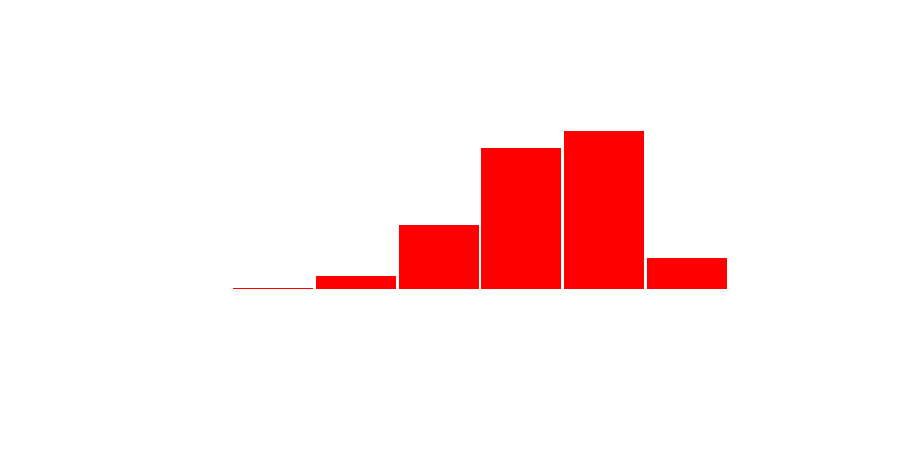
\includegraphics[scale = 0.1, clip = true, trim= 50px 60px 50px 60px]{hist-6b5159d3060b4fdf8493d4c818f79949.pdf} \\ 
  \texttt{team\_size} & Number of active core team members during the last 3 months prior to the pull request creation. & 1.00 & 15.37 & 7.00 & 65.00 & 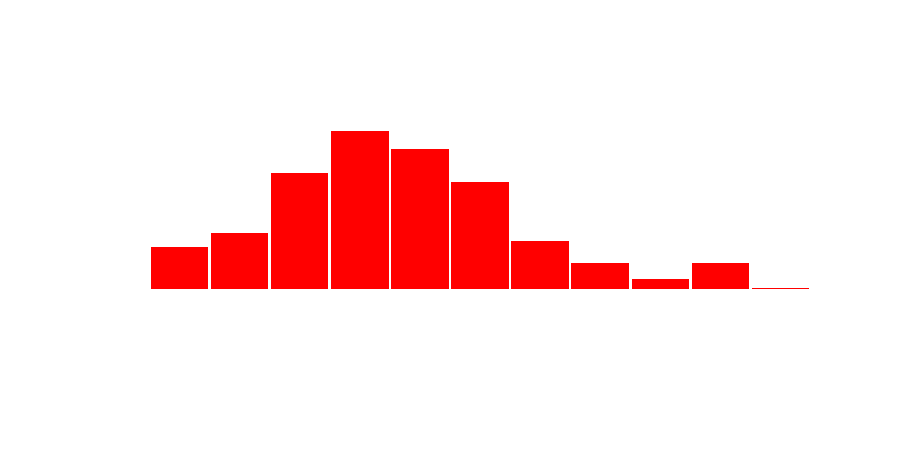
\includegraphics[scale = 0.1, clip = true, trim= 50px 60px 50px 60px]{hist-231fb4fabf4a3f0c551f2a97ae080508.pdf} \\ 
  \texttt{perc\_ext\_contribs} & The ratio of commits from external members over core team members in the last 3 months. & 8.00 & 52.81 & 54.00 & 95.00 & 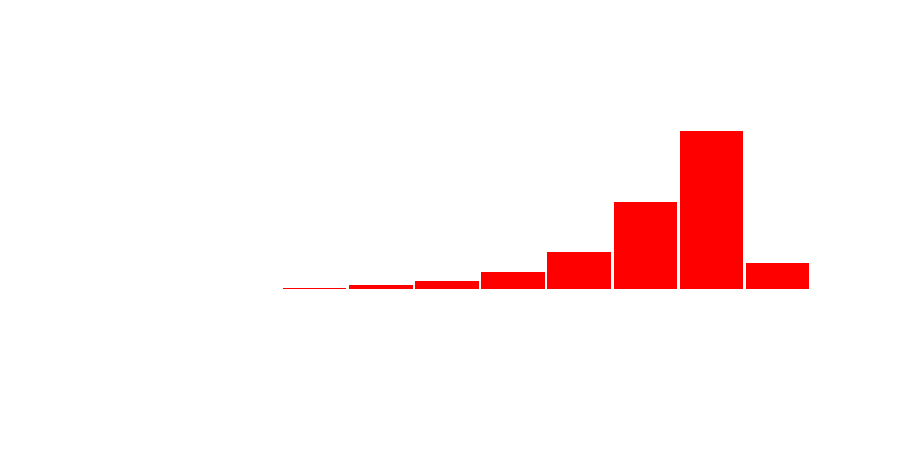
\includegraphics[scale = 0.1, clip = true, trim= 50px 60px 50px 60px]{hist-a222f0a5c377ba129dd6c8f257062591.pdf} \\ 
  \texttt{commits\_files\_touched} & Number of total commits on files touched by the pull request 3 months before the pull request creation time. & 0.00 & 52.39 & 5.00 & 210.00 & 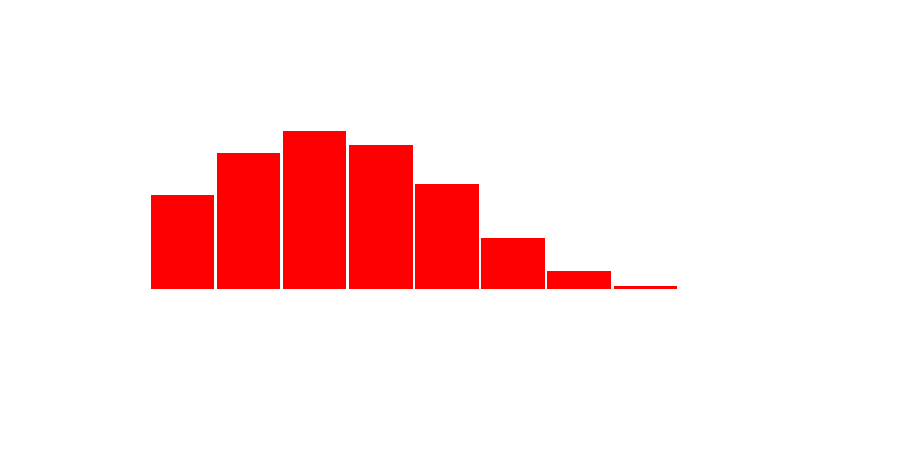
\includegraphics[scale = 0.1, clip = true, trim= 50px 60px 50px 60px]{hist-b735900ffcc37e7eda16dcd0c3497e6e.pdf} \\ 
  \texttt{test\_lines\_per\_kloc} & A proxy for the project's test coverage. & 1.39 & 1,002.61 & 440.80 & 2,147.43 & 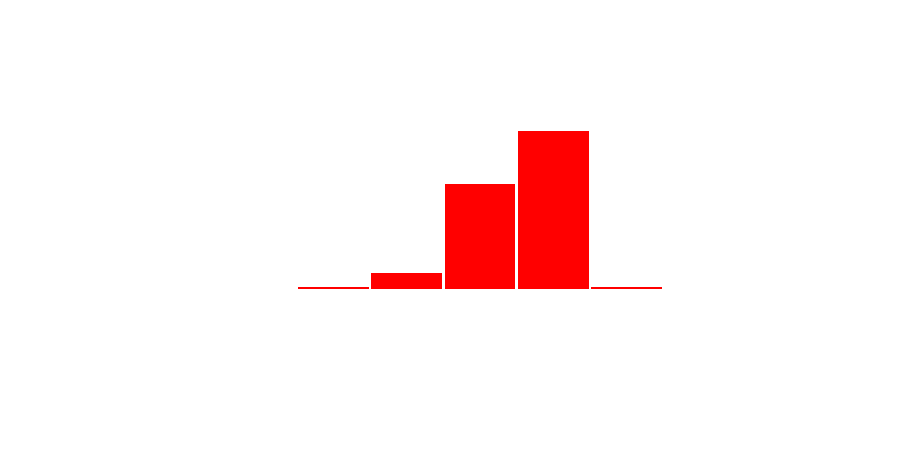
\includegraphics[scale = 0.1, clip = true, trim= 50px 60px 50px 60px]{hist-67ff3047089ba9ce0528884eab66e80a.pdf} \\ 

  \multicolumn{2}{l}{\bf{Developer}}\\

  \texttt{prev\_pullreqs} & Number of pull requests submitted by a specific developer, prior to the examined pull request. & 0.00 & 45.11 & 14.00 & 195.00 & 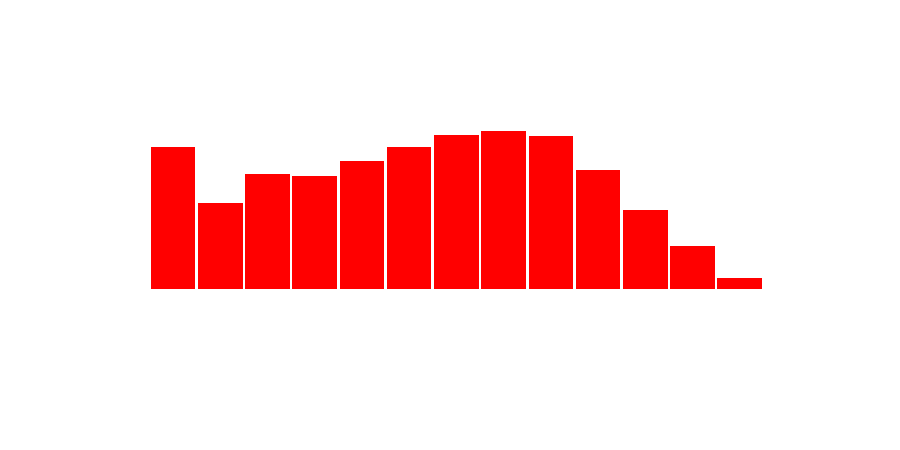
\includegraphics[scale = 0.1, clip = true, trim= 50px 60px 50px 60px]{hist-a2f7f60851dfa13cfbe0227d1d233767.pdf} \\ 
  \texttt{requester\_succ\_rate} & \% of the developer's pull requests that have been merged up to the creation of the examined pull request. & 0.00 & 0.59 & 0.78 & 1.00 & 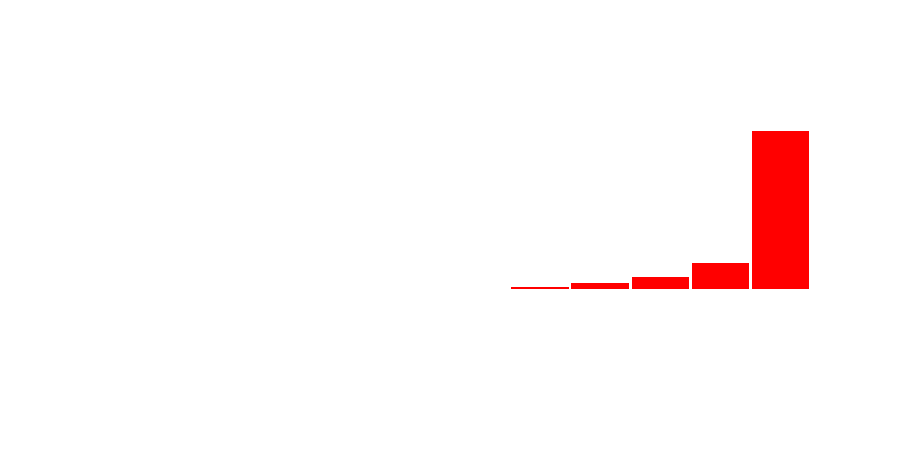
\includegraphics[scale = 0.1, clip = true, trim= 50px 60px 50px 60px]{hist-9363017165c3ded62457750f1c67c1af.pdf} \\ 
   \hline
\end{tabular}
\end{small}
\label{tab:features}
\end{table*}


\paragraph*{Merge detection}
To identify pull requests that are merged outside Github, we resorted to
the following heuristics, listed here in order of application:

\begin{compactdesc}

  \item[$H_1$] At least one of the commits associated with the pull request appears in the target project's master branch.

  \item[$H_2$] A commit closes the pull request (using the \texttt{fixes:}
    convention advocated by Github) and that commit appears in the project's
    master branch.  This means that the pull request commits were squashed onto
    one commit and this commit was merged.

  \item[$H_3$] One of the last 3 (in order of appearance) discussion comments
    contain a commit unique identifier, this commit appears in the project's
    master branch and the corresponding comment can be matched by the following
    regular expression:

    \begin{small}
    \texttt{(?:merg|appl|pull|push|integrat)(?:ing|i?ed)}
    \end{small}

  \item[$H_4$] The latest comment prior to closing the pull request matches the
    regular expression above.

\end{compactdesc}

If none of the above heuristics identifies a merge, the pull request is
identified as unmerged. The heuristics proposed above are not complete, i.e. they may not identify all merged pull requests, nor sound, i.e. they might lead to false positives (especially $H_4$).

\paragraph*{Test case detection}
In \emph{Ruby} projects, files under the \texttt{/test/} and \texttt{/spec/}
directories are considered test files. Test cases are recognized by scanning
through the test files lines for method name patterns as required by the
\textsf{RUnit}, \textsf{Rspec}, \textsf{Shoulda} and \textsf{Minitest}
frameworks. The popular Cucumber behaviour driven development testing framework
is excluded from the analysis due to inexistent naming conventions.  In
\emph{Python}, project conventions do not specify specific directories for test
files, so test file detection is based solely on whether the file name contains
the word ``test'' as prefix or suffix. Test cases and asserts are discovered
both in source code and also in API examples embedded in documentation comments
(also known as \emph{doctests}).

Following Maven conventions, in \emph{Java} projects, files in directories under
a \texttt{test/} branch of the file tree are considered test files.
\textsf{junit4} test cases are recognized using the \texttt{@Test} tag. For
\textsf{junit3}, methods starting with test are considered as test methods.
Asserts are counted by searching through the source code lines for
\texttt{assert} statements. Finally, as Maven underlies \emph{Scala}'s default
build system (\textsf{sbt}), the same conventions as in the Java case can be
used to discover test files. In addition to \textsf{junit}, the process can
discover test cases and assert statements as defined by the \textsf{scalatest}
and \textsf{specs2} testing frameworks.


\paragraph*{Counting lines, files and file types}

In the \pullreqs dataset, a line of code is an executable statement,
excluding blank lines and comments. To measure lines, we developed custom
comment strippers for all the programming languages the dataset supports, as
we could not find any tool that can count lines reliably (block comments in Ruby and Python were a particular problem).
Moreover, we delegated the identification of file types to a Ruby library
called Linguist (the same that Github uses), which supports more than 250 file types.

\paragraph*{Further Quality Control}
After the dataset was constructed, the following criteria were applied to 
ensure homogeneity:

\begin{compactitem}

  \item The number of pull requests in the data files should be more
    that 70\% of the pull requests in the database.
    The typical reason for some pull requests missing from the output
    is that many projects use a dedicated branch for documentation which
    includes no source code; the data generation script skips such pull
    requests. Other reasons might include the project has been deleted from
    Github or no source code files could be identified in a specific version. 
    119 projects were filtered out.

  \item The ratio of merged pull requests should be within reasonable limits
    from the mean merge ratio across all Github projects. In the \ghtorrent
    dataset, the mean merge ratio is 72\%. The \pullreqs dataset uses heuristics
    to identify merges done outside Github, so we generally expect a mean merge
    ratio close to or higher of the one across Github. For this reason, 
    we filtered out the lowest 5\% of the projects. The remaining projects
    exhibit a merge ratio more than 50.8\%. 43 projects were filtered out.

\end{compactitem}

\paragraph*{Results} The final dataset consists of 865 projects (303 Python, 253 Java, 274 Ruby, 35 Scala) and 336,502 pull requests (120,475; 83,960; 113,665 and 18,402 for Python,
Ruby, Java and Scala pro\-je\-cts respectively). 60\% of the pull requests are
merged using Github's facilities while 16\% are identified as unmerged.
The remaining 24\% is identified as merged using the heuristics described
above ($H_1$: 11\%, $H_2$: 3\%, $H_3$: 4\%, $H_4$: 6\%).
Moreover, as Figure~\ref{fig:features} shows,
the selected features are fairly orthogonal, with very few strong correlations
between them. This indicates that they capture a wide range of pull
request activities with minimal overlap.

\section{Tools}

The \pullreqs dataset is accompanied by an extensive analysis toolkit written in
the R statistics language. The framework allows researchers to load selections
of projects in R, provides basic statistics in tabular (e.g.
Table~\ref{tab:features}) and graphical form (e.g. Figure~\ref{fig:features}),
and exposes a command line base interface that tools can extend. Moreover, it
implements a modular, multi-step data mining framework that researchers can
easily re-use in similar machine learning experiments. The data mining parts
include all the necessary steps for successfully executing a data mining
experiment, such as distribution plotting, cross correlation among features,
pluggable model and algorithm definitions, $n$-fold cross-validation and
plotting of important model variables such as Area Under Curve ({\sc auc}) and
accuracy across cross-validation runs. To cope with the \pullreqs dataset size,
several parts of the tooling (mainly the cross validation and variable
importance steps) employ parallelism and can thus exploit multi-core machines.

\section{Limitations}

The dataset, while extensive, is not entirely representative of all pull request
activity on Github. Specifically, while it covers almost 10\% of the pull
requests available in the GHTorrent database, the project selection process and
consequent filtering leave out important aspects (e.g. development in
Javascript, the most popular language on Github). Moreover, to analyze the
projects, we extracted data from i) the {\sc ght}orrent relational database ii)
the {\sc ght}orrent raw database iii) each project's Git repository.
Differences in the data abstraction afforded by each data source may lead to
different results in the following cases: i) Number of commits in a pull
request: During their lifecycle, pull requests may be updated with new commits.
However, when developers use commit squashing, the number of commits is reduced
to one. Therefore the number of commits feature is often an idealized version of
the actual work that took place. ii) Number of files and commits on touched
files: The commits reported in a pull request also contain commits that merge
branches, which the developer may have merged prior to performing his changes.
These commits may contain several files not related to the pull request itself,
which in turn affects our results. We  filtered out such commits, but this may
not reflect the contents of certain pull requests.

\section{Related Work}
\label{sec:rel}

The \pullreqs dataset is similar to the code review datasets published by
Hamasaki et al.~\cite{Hamas13} and Mukadam et al.~\cite{Mukad13}.  While code
reviewing is an inherent characteristic of pull requests, pull requests cover a
wider range of project activities, such as discussion on project features,
integration of attached external tools (continuous integration, code quality
evalaution), management of project goals through milestones etc.  Thus the
\pullreqs dataset improves upon those two datasets not only by covering a wider
array of projects and languages but also by offering more precise related data,
such as file counts and test cases and covering a wider range of activities. To
the best of our knowledge, this is the only publicly available dataset covering
pull-based development and certain aspects of distributed software development
in general.

\section{Research Opportunities}

The \pullreqs dataset can be used for a multitude of studies, apart from basic
exploration of the pull-based distributed development model. Making the pull
request process more efficient requires research in topics such as \emph{pull
request triaging} and \emph{patch quality evaluation}.  Tools that recommend
appropriate developers for doing code reviews or label pull requests according
to their characteristics might be possible. The dataset can then be used as a
benchmark for comparing recommender systems. \emph{Code reviews} are a core
ingredient of the pull request model. Using this dataset, a researcher can
readily get quantitative data for thousands of code reviews, which can then be
combined with qualitative data for specific projects.  Finally, Github has been
praised for lowering the entry barrier for casual contributions to projects, but
do projects actually take advantage of this? \emph{Community openess} is an
important property for projects hosted on Github; the \pullreqs dataset can be
used to evaluate aspects of it.

We presented the \pullreqs dataset, a curated dataset of almost 900 projects,
along with a statistical tool set for its analysis. The
dataset itself can be extended to support more programming languages and more
projects. All source code and data is available on the Github repository
\href{https://github.com/gousiosg/pullreqs}{gousiosg/pullreqs}. Data on the
\href{http://ghtorrent.org}{ghtorrent.org} web site permit full replication
of the construction process or the expansion of this dataset.
Pull requests are especially welcome!

\section{Acknowledgements}
This work is supported by the {\sc nwo} 639.022.314 --- TestRoots project.

\bibliographystyle{abbrv}
\balance
%\begin{small}

  \bibliography{dataset}
%\end{small}

\end{document}
